\chapter{基于移动模式最优节点群组选取的路由算法}

在许多节点具有一定社会属性的机会网络中,具有共同兴趣的移动用户往往访问一些与其兴趣相关的地点。研究表明,50\%的移动用户会在某一个特定的接入点(access point, AP)上花费约74\%的时间\cite{Henderson:2004ul}。换言之,节点往往具有频繁访问某一或某一部分地点(简称为常访地点)的特点。这些常访地点可被看做``连接''这些节点的枢纽。可以通过在常访地点部署缓存设备,用以辅助消息传递,例如投掷盒(throw-box)\cite{Ibrahim:2009we}等设备。缓存设备具有普通移动节点不具备的优势。首先,由于部署的缓存设备位置固定在常访地点,且节点往往在常访地点停留一段时间,所以节点与缓存设备之间具有比移动节点之间更加稳定的连接。其次,这些固定的缓存设备,没有如同移动节点那样便携性的限制和要求,故其存储容量往往比移动节点要大许多。由此,可以利用在常访地点部署缓存设备作为中继枢纽,从而提升机会网络中路由算法的性能表现。

本章研究多副本单播机会路由算法,基本假设如下。每条消息具有一对“源—目的”节点对(source-destination node pair),并且每条消息可在网络中具有多份拷贝。不同于以往基于社会网络分析求解社会关系的方法,或自定义社会属性的方法,本章利用节点收集的移动记录信息,从中提取出节点(群组)移动模式,并以此为依据选出最优中继节点群组。基本思想为:将持有某一条特定消息(或其拷贝)的任意一组节点看成一个整体,从记录信息中提取出移动模式,从而确定该节点群组的常访地点集合$A_1$。目的节点的常访地点$A_2$,也以相同方法获取。进而,取交集求得$A=A_1\cap A_2$,作为该节点群组与目的节点的共同常访地点集合。利用集合$A$,可以求出消息的预测投递率。路由目标即为求得能使预测投递概率最大的节点群组。此外,超出有效期(deadline)的消息不再具有价值,在求解移动模式的过程中,消息的时效性也被考虑在内。本章基于节点的移动模式,提出构造最优节点群组作为中继节点群的移动模式相关最优路由算法(Movement Pattern-Aware optimal Routing, MPAR)。就目前掌握的资料来看,这是首次利用节点群组移动模式进行社会相关的路由算法研究。

本章组织如下:第\ref{chap3:系统模型及基本定义}节引入系统模型及基本定义;第\ref{chap3:路由问题概览}节分析路由问题背后蕴含的两个关键属性,并给出最优路由问题的形式化定义;第\ref{chap3:搜索问题分析}节证明了该最优问题的计算复杂性,并提出了启发式算法用以求解近似最优解;第\ref{chap3:最优化路由算法}节给出路由算法的详细过程及描述;第\ref{chap3:仿真实验}节对仿真实验结果进行分析;第\ref{chap3:总结}节总结本章内容。

\section{系统模型及基本定义}
\label{chap3:系统模型及基本定义}

\subsection{网络模型}

网络节点集合记为$\overline{N}\triangleq\{n_i|1\leq i\leq n\}$. 节点在给定的地点集合间移动,地点集合记为$\overline{A}\triangleq\{a_j|1\leq j \leq m\}$. 任意一个节点$n_i$的常访地点集合$A(n_i)\subseteq \overline{A}$. 该模型源于真实的移动网络,一个典型的实例是Dartmouth College的Wi-Fi Campus Network \cite{Jedari:2013uo}。另一符合该模型的一类网络是VANET。在VANET中,大量的公交车,电车等在车站等固定地点间移动。我们假设节点$n_i$访问任意一个地点$a_j$的时间间隔服从指数分布。此外,在任意地点内都部署有一个投掷盒装置,用于接受,缓存及传递消息。在此模型中,投掷盒的缓存容量假设为足够大,即在投掷盒中不会因缓存满而产生消息丢弃。如\figurename~\ref{fig:chap3_box}所示,节点a在$t_1$时刻将消息托管给投掷盒,在$t_2$时刻,该消息的目的节点d进入投掷盒的传输范围内,并从投掷盒接受该消息,至此,消息的投递操作完成。

我们假设每条消息$l$都具有一个值$\tau_l$,代表消息$l$在网络的剩余生存时间。随着时间消逝,$\tau_l$的值逐渐减少,当$\tau_l=0$时,该消息将从节点缓存中删除,不再存在于网络中。消息的生存时间属性,一定程度上避免了消息在网络中停留的时间过长。此外,应用程序所产生的消息因具有时效性,往往也会对消息设定一个生存时间。例如新闻发布或者广告发布服务,消息只在一定时间内有效。当消息超出某个时间即不再具有投递价值。

\begin{figure}
\centering
\subfigure[节点a向投掷盒发送消息\label{paper-MPAR/send_to_box}]
{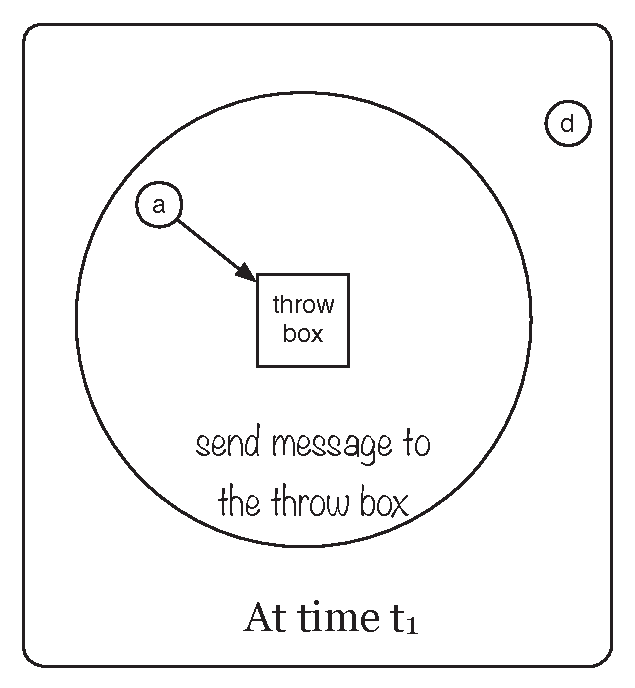
\includegraphics[width=0.4\linewidth]{paper-MPAR/send_to_box}}~~~~~~
\subfigure[节点d从投掷盒接受消息\label{paper-MPAR/receive_from_box}]
{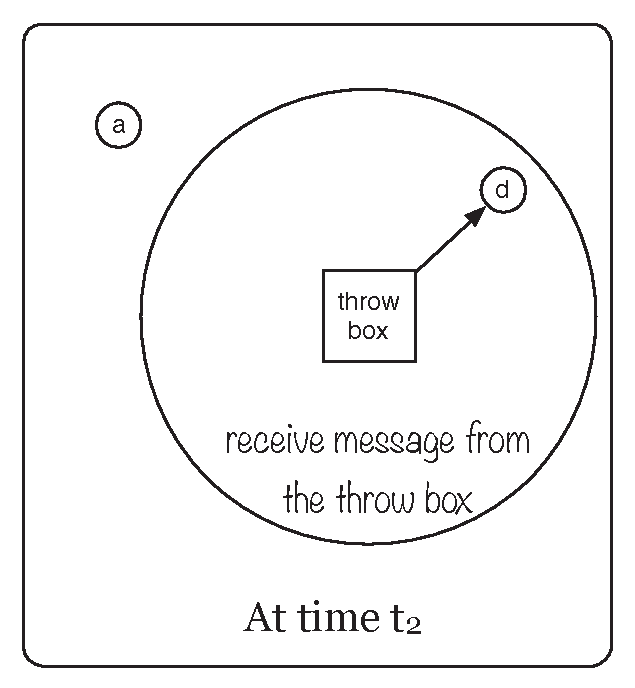
\includegraphics[width=0.4\linewidth]{paper-MPAR/receive_from_box}}
\caption{利用投掷盒完成消息从节点a到节点d的传递操作.}
\label{fig:chap3_box}
\end{figure}


\subsection{基本定义}

由于作为手持设备的节点附属于具有社交属性的人群,节点的移动模式具有一定的周期性。举例而言,Smith先生在周一到周五上班,故其常访地点可能包含家,办公室,某些公交站点及一些快餐店等。周末,Smith先生通常去健身俱乐部或咖啡馆,或者一些不同于工作时间去的地方。然而,他的行为通常以一星期为一个周期,在一定程度上重复,即其移动记录具有一定的周期性。假设周期为$T$,若将$T$划分为$h$个时间槽,则每个时间槽的长度为$\frac{T}{h}$。将这些划分好的时间槽的边界时间点,用序列$<t_0,t_1,t_2,\ldots,t_h>$表示,则任意两个区间点$t_s$与$t_e$($t_s<t_e$)形成时间区间$[t_s,t_e]$,如图\figurename~\ref{fig:chap3_time_slots}所示。针对时间区间$[t_s,t_e]$,可以从节点的移动记录中,提取出对应的移动模式。节点的移动记录见定义\ref{def:移动记录}。

\begin{figure}[!t]
\centering
  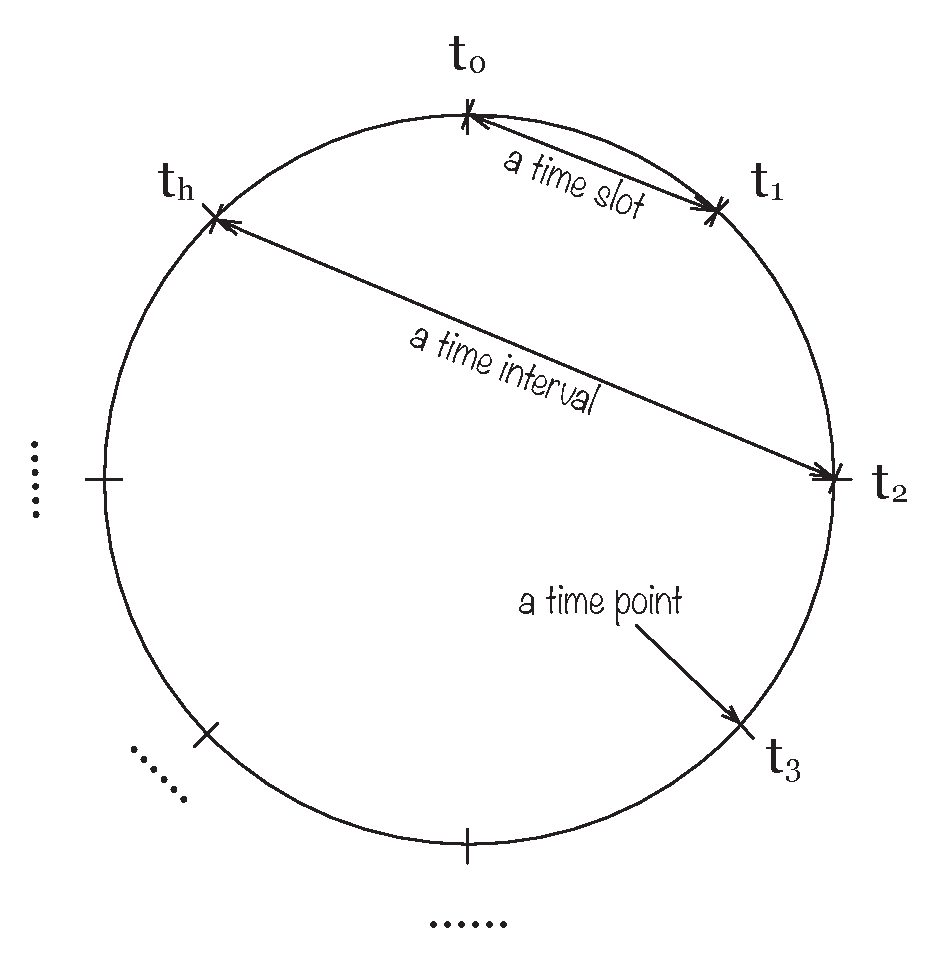
\includegraphics[width=0.55\linewidth]{paper-MPAR/time_slots}
  \caption{周期$T$划分为$h$个时间槽}
  \label{fig:chap3_time_slots}
\end{figure}

\begin{definition} 移动记录\\
节点$n_i$的移动记录定义为一个$h\times m$矩阵,记为$\mathbb{R}(i)$
\[
\mathbb{R}(i)=
\left.\left[
\overbrace{
\begin{array}{cccc}
\sfrac{1}{r_{1,1}^i} & \sfrac{1}{r_{1,2}^i} & \ldots & \sfrac{1}{r_{1,m}^i}\\
\sfrac{1}{r_{2,1}^i} & \sfrac{1}{r_{2,2}^i} & \ldots & \sfrac{1}{r_{2,m}^i} \\
\vdots & \vdots & \ddots & \vdots \\
\sfrac{1}{r_{h,1}^i} & \sfrac{1}{r_{h,2}^i} & \ldots & \sfrac{1}{r_{h,m}^i} \\
\end{array}}^{m\textnormal{个地点}}
\right]\right\}\small{h\textnormal{个时间槽}}
\]
其中第$k$行的向量$\mathbb{R}(i,k)$代表时间槽$[t_{k-1},t_{k}]$内的移动记录,且有\[\mathbb{R}(i,k)=[\sfrac{1}{r^i_{k,1}},\sfrac{1}{r^i_{k,2}},\ldots,\sfrac{1}{r^i_{k,m}}]\]其中$r^i_{k,j}$代表节点 $n_i$对地点$a_j$在时间槽$[t_{k-1},t_{k}]$内的平均访问时间间隔。
\label{def:移动记录}
\end{definition}

从上述定义可知,$\sfrac{1}{r^i_{k,j}}$代表节点$n_i$对地点$a_j$的平均访问频率。特别的,若$n_i$在时间槽$[t_{k-1},t_k]$内从未到达过$a_j$,则设定$r_{k,j}^i=\infty$,于是有$\sfrac{1}{r^i_{k,j}}=0$. 对于所有的时间槽,可以求出节点$n_i$对于地点$a_j$的平均访问时间间隔$M_{i,j}$,记为
\begin{equation}
M_{i,j}=\left.\sum_{k=1}^{k=h}r^{i}_{k,j}\middle/h\right.
\label{eq:meeting_interval}
\end{equation}

\section{路由问题概览}
\label{chap3:路由问题概览}

在讨论路由相关细节之前,先对路由问题做一个总览。在\ref{chap3:移动模式}小节中,讨论如何从一组节点中提取对应的节点群组移动模式。随后在\ref{chap3:路由相关的两个关键属性}小节中,分析路由相关的两个关键属性。最后,在\ref{chap3:路由问题形式化定义}小节中,给出最优路由问题的形式化定义。

\subsection{移动模式}
\label{chap3:移动模式}

移动模式从节点的移动记录中提取。首先定义函数$\mathbbm{E}$,用以将移动记录向量转化为对应的移动模式向量。

\begin{figure}[hbt]
\centering
  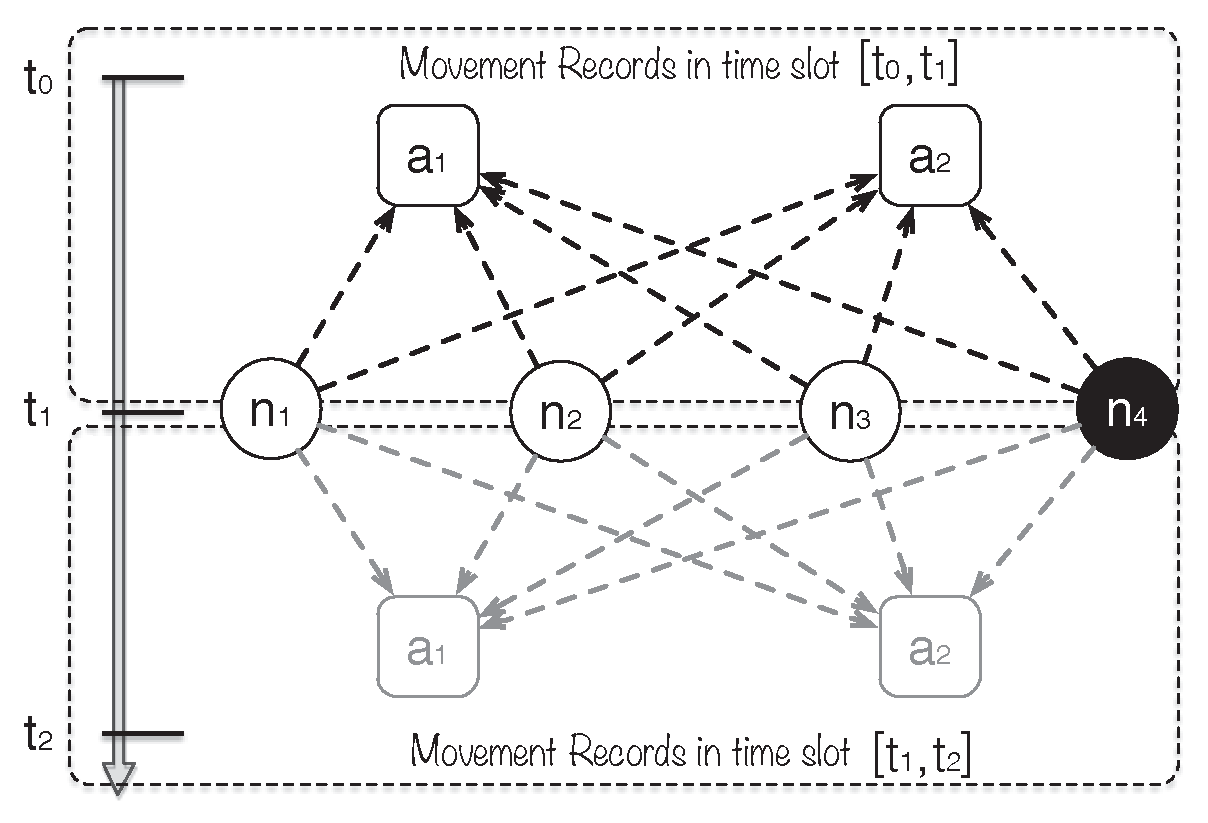
\includegraphics[width=0.5\linewidth]{paper-MPAR/example1}
  \caption{网络场景举例}
  \label{fig:chap3_example1}
\end{figure}

\begin{definition} 函数$\mathbbm{E}$
\[\mathbbm{E}([x_1,x_2,\ldots,x_m])=[\varkappa _1,\varkappa _2,\ldots,\varkappa _m]\]\textnormal{其中}
\begin{equation}
\varkappa _j=\left\{
\begin{array}{cl}
 1 &x_j\geq\frac{\updelta}{m}\sum_{i=1}^{i=m}x_i\\
 0 & otherwise
\end{array}
\right.
\label{eq:extract}
\end{equation}
\textnormal{$0<\updelta<1$ 是预设的系统参数。}
\label{def:函数E}
\end{definition}

函数$\mathbbm{E}$用于过滤节点—地点间的访问记录,不常访问的地点将被过滤掉。基于函数$\mathbbm{E}$可以直接定义移动模式,如定义\ref{def:移动模式}。

\begin{definition} 移动模式.
对于任意节点群组$N$,其在时间区间$[t_p,t_q]$ 内的移动模式,记为$\mathcal{P}(V,[t_s,t_e])$, 定义为
\begin{equation}
\mathcal{P}(N,[t_s,t_e])= \mathbbm{E}(\sum_{n_x \in N}\sum_{i=s}^{i=e}\mathbb{R}(x,t_i))
\label{eq:pattern}
\end{equation}
\label{def:移动模式}
\end{definition}

在定义\ref{def:移动模式}中,移动模式$\mathcal{P}$从某节点(群组)在某个特定时间区间$[t_s,t_e]$上的所有移动记录向量通过累加后,以函数$\mathbbm{E}$处理后得出。举例而言,假设如\figurename~\ref{fig:chap3_example1}所示的网络场景,网络中总共有四个节点$n_1,n_2,n_3,n_4$以及两个地点$a_1,a_2$。其中$n_4$是目的节点,周期$T$被划分为两个时间槽,简记为$[t_0,t_1]$与$[t_1,t_2]$。



\figurename~\ref{fig:chap3_example1}中每条边的权值如\tablename~\ref{tab:chap3_example1}所示。权值代表“节点—地点”对访问平均间隔时间。针对每个节点的记录矩阵,表示为$\mathbb{R}(1),\mathbb{R}(2),\mathbb{R}(3),\mathbb{R}(4)$。

\[
\begin{array}{cc}
\mathbb{R}(1)=\left[
\begin{array}{cc}
\sfrac{1}{2.08} & \sfrac{1}{4.65} \\
\sfrac{1}{6.02} & \sfrac{1}{2.95}
\end{array}\right]&
\mathbb{R}(2)=\left[
\begin{array}{cc}
\sfrac{1}{4.4} & \sfrac{1}{4.3} \\
\sfrac{1}{4.0} & \sfrac{1}{4.5}
\end{array}\right]    \\ \\
\mathbb{R}(3)=\left[
\begin{array}{cc}
\sfrac{1}{8.05} & \sfrac{1}{1.11} \\
\sfrac{1}{6.05} & \sfrac{1}{15.49}
\end{array}\right]
&
\mathbb{R}(4)=\left[
\begin{array}{cc}
\sfrac{1}{2.6} & \sfrac{1}{3.3} \\
\sfrac{1}{3.5} & \sfrac{1}{3.5}
\end{array}\right]
\end{array}
\]

\begin{table}[hbt]
\centering
  \caption{网络场景\figurename~\ref{fig:chap3_example1}边权值}
  \begin{tabular}{|c|c|cc|}
  \hline
    & & $a_1$ & $a_2$  \\
    \hline
    
    %%t1
    \multicolumn{1}{|c|}{\multirow{4}{*}{$[t_0,t_1]$}} & $n_1$ &2.08 & 4.65 \\
    & $n_2$ & 4.4 & 4.3 \\
    & $n_3$ & 8.05 & 1.11 \\
    & $n_4$ & 2.6 & 3.3 \\
    \hline

    %%t2
    \multicolumn{1}{|c|}{\multirow{4}{*}{$[t_1,t_2]$}} & $n_1$ &6.02 & 2.95 \\
    & $n_2$ & 4.0 & 4.5 \\
    & $n_3$ & 6.05 & 15.49 \\
    & $n_4$ & 3.5 & 3.5 \\
    \hline
  \end{tabular}
  \label{tab:chap3_example1}
\end{table}
节点集合$\{n_1,n_2,n_3\}$的移动模式,可以利用公式\ref{eq:pattern}从对应的移动记录中提取出来。对应的移动记录累加计算如下:
\begin{multline*}
\sum_{i=1}^{i=3}\sum_{j=1}^{j=2}\mathbb{R}(i,j) = \left[\frac{1}{2.08}+\frac{1}{4.4}+\frac{1}{8.05}+\frac{1}{6.02}+\frac{1}{4.0}+\frac{1}{6.05},\right.\\
\left.\frac{1}{4.65}+\frac{1}{4.3}+\frac{1}{1.11}+\frac{1}{2.95}+\frac{1}{4.5}+\frac{1}{15.49}\right]= [1.414,1.974]
\end{multline*}
针对公式\ref{eq:extract},设定参数$\delta=0.95$,从定义\ref{def:函数E}得出
\[
\frac{\updelta}{m}\sum_{i=1}^{i=m}v_i=\frac{0.95}{2}\times(1.414+1.974)\approx 1.609
\] 
所得值1.609大于向量第一个元素值1.414,且小于向量第二个元素值1.974,故对应移动模式提取如下
\[
\mathcal{P}(\{n_1,n_2,n_3\},[t_0,t_2])=[0,1] 
\]

移动模式$\mathcal{P}$指明了节点群组$\{n_1,n_2,n_3\}$在时间区间$[t_0,t_2]$内的的常访区域集合,即$A(\{n_1,n_2,n_3\},[t_0,t_2])=\{a_2\}$。对于集合$\overline{N}\\\{n_d\}$,共有$2^{n-1}-1$个非空子集,每一个子集可被看做用于向目的节点$n_d$合作投递消息的一个整体。在本例中,基于移动记录,提取出非空节点集$\{n_1,n_2,n_3\}$以及目的节点$n_4$的移动模式,结果如下。

\begin{tabular}{ll}
 & \\
$\mathcal{P}(\{n_1\},[t_0,t_2])=[1,0]$ & $\mathcal{P}(\{n_1,n_2\},[t_0,t_2])=[1,0]$ \\
$\mathcal{P}(\{n_2\},[t_0,t_2])=[1,1]$ & $\mathcal{P}(\{n_1,n_3\},[t_0,t_2])=[0,1]$ \\
$\mathcal{P}(\{n_3\},[t_0,t_2])=[0,1]$ & $\mathcal{P}(\{n_2,n_3\},[t_0,t_2])=[0,1]$ \\
$\mathcal{P}(\{n_4\},[t_0,t_2])=[1,1]$ & $\mathcal{P}(\{n_1,n_2,n_3\},[t_0,t_2])=[0,1]$ \\
 &
\end{tabular}

对应的常访地点集合,如下。

\begin{tabular}{ll}
 & \\
$A(\{n_1\},[t_0,t_2])=\{a_1\}$ & $A(\{n_1,n_2\},[t_0,t_2])=\{a_1\}$ \\
$A(\{n_2\},[t_0,t_2])=\{a_1,a_2\}$ & $A(\{n_1,n_3\},[t_0,t_2])=\{a_2\}$ \\
$A(\{n_3\},[t_0,t_2])=\{a_2\}$ & $A(\{n_2,n_3\},[t_0,t_2])=\{a_2\}$ \\
$A(\{n_4\},[t_0,t_2])=\{a_2\}$ & $A(\{n_1,n_2,n_3\},[t_0,t_2])=\{a_1,a_2\}$ \\
 &
\end{tabular}

\subsection{路由相关的两个关键属性}
\label{chap3:路由相关的两个关键属性}

\subsubsection{投递概率}

设节点集合$N$在时间区间$[t_0,t_0+t_l]$内的移动模式为$P(N,[t_0,t_0+t_l])$,目的节点$n_d$的移动模式为$\mathcal{P}(n_d,[t_0,t_0+\tau_l])$,共同常访地点集合记为$A$,则有$A=A(N,[t_0,t_0+\tau_l])\cap A(n_d,[t_0,t_0+\tau_l])$。记任意地点$a_j$及任意节点$n_i\in N$满足节点$n_i$和$n_d$
都在某一时间访问$a_j$。设随机变量$T_{i,j}$及$T_{d,j}$分别代表$n_i$和$n_d$到达$a_j$的时间,若要使消息能够成功传递,则须满足$T_{i,j}<T_{d,j}<\tau_l$,换言之,$n_i$须先于$n_d$到达$a_j$托管消息,且$n_d$需在消息到期之前到达$a_j$取出消息。为了便于讨论,设起始时间点$t_0=0$。此外,如\ref{chap3:系统模型及基本定义}节所述,任意节点访问任意地点的时间间隔服从指数分布。从公式\ref{eq:meeting_interval}可以计算出节点$n_i$访问地点$a_j$的指数分布参数$\lambda_{i,j}$,即

\[
\lambda_{i,j} = \sfrac{1}{M_{i,j}}
\]

对于$A$为空集的情形,默认其预测投递概率为0,到达其它地点的期望时延为$\infty$。对于$A$非空的情形,可依公式(\ref{eq:probability})预测节点$n_i$对$n_d$的投递率。进一步的,节点集$N$对$n_d$的投递率可依公式(\ref{eq:probability2})预测。
\begin{multline}
P_{i,d}=1-\prod_{a_j\in A}\left(1-P(T_{i,j}<T_{d,j}<\tau_l) \right) \\
=1-\prod_{a_j\in A}\left(1-\int _{0}^{\tau _l}\!\!\!\!\int _{t_{i,j}}^{\tau _l}f_{T_{i,j},T_{d,j}}\left(t_{i,j},t_{d,j}\right)dt_{d,j}dt_{i,j}\right)\\
=1-\prod_{a_j\in A}\left(1-\int _{0}^{\tau _l}\!\!\!\!\int _{t_{i,j}}^{\tau _l}f_{T_{i,j}}(t_{i,j})f_{T_{d,j}}(t_{d,j}) dt_{d,j}dt_{i,j}\right) \\
=1-\prod_{a_j\in A}\left(1-\int _{0}^{\tau _l}\!\!\!\!\int _{t_{i,j}}^{\tau _l}\lambda _{d,j} \lambda _{i,j} e^{-\left(\lambda _{d,j}t_{d,j}+\lambda _{i,j}t_{i,j}\right)}dt_{d,j}dt_{i,j}\right)\\
=1-\prod_{a_j\in A}\left(1-\frac{\lambda _{i,j} \left(1-e^{-\tau _l \left(\lambda _{d,j}+\lambda _{i,j}\right)}\right)}{\lambda _{d,j}+\lambda _{i,j}}
-\left(e^{\tau _l \lambda _{i,j}}-1\right) e^{-\tau _l \left(\lambda _{d,j}+\lambda _{i,j}\right)}\right)
\label{eq:probability}
\end{multline}
\begin{multline}
P_{N,d}=1-\prod_{n_i\in N}(1-P_{i,d}) \\
=1-\prod_{n_i\in N}\prod_{a_j\in A}\left(1-\frac{\lambda _{i,j} \left(1-e^{-\tau _l \left(\lambda _{d,j}+\lambda _{i,j}\right)}\right)}{\lambda _{d,j}+\lambda _{i,j}}
-\left(e^{\tau _l \lambda _{i,j}}-1\right) e^{-\tau _l \left(\lambda _{d,j}+\lambda _{i,j}\right)}\right)
\label{eq:probability2}
\end{multline}
特别而言,当消息生存时间设为无穷时,即$\tau_l=\infty$,有
\begin{multline}
P_{i,d} = 1-
\prod_{a_j\in A}\left(1-\int _0^{\infty }\!\!\!\!\int _{t_{i,j}}^{\infty }\lambda _{d,j} \lambda _{i,j} e^{-\left(\lambda _{d,j} t_{d,j}+\lambda _{i,j} t_{i,j}\right)}dt_{d,j}dt_{i,j} \right)\\
=1-\prod_{a_j\in A}\left(1-\frac{\lambda _{i,j}}{\lambda _{d,j}+\lambda _{i,j}}\right)
\label{eq:probability_infty}
\end{multline}
对于$P_{N,d}$,有
\begin{equation}
P_{N,d} = 1-\prod_{n_i\in N}\prod_{a_j\in A}\left(1-\frac{\lambda _{i,j}}{\lambda _{d,j}+\lambda _{i,j}}\right) 
=1-\prod_{n_i\in N}\prod_{a_j\in A}\frac{\lambda _{d,j}}{\lambda _{d,j}+\lambda _{i,j}}
\label{eq:probability2_infty}
\end{equation}


\subsubsection{期望时延}

\subsection{路由问题形式化定义}
\label{chap3:路由问题形式化定义}

\section{$N_{opt}$搜索问题分析}
\label{chap3:搜索问题分析}

\subsection{计算复杂性证明}

\subsection{局部陷阱}

\subsection{基于禁忌搜索的求解方法}

\section{最优化路由算法}
\label{chap3:最优化路由算法}

\subsection{Local-MPAR:基于局部搜索的路由算法}

\subsection{Tabu-MPAR:基于禁忌搜索的路由算法}

\section{仿真实验}
\label{chap3:仿真实验}

\subsection{自变量:消息生存时间}

\subsection{自变量:节点缓存}

\section{结论}
\label{chap3:结论}






